\documentclass[10pt,a4paper]{article}

\usepackage[a4paper,margin=2.25cm,headheight=14pt]{geometry}
\usepackage[T1]{fontenc}
\usepackage[utf8]{inputenc}
\usepackage{lmodern}
\usepackage{microtype}
\usepackage{amsmath,amssymb,mathtools}
\usepackage{booktabs,array,tabularx,multirow}
\usepackage{graphicx}
\usepackage{xcolor}
\usepackage{enumitem}
\usepackage{listings}
\usepackage{caption}
\usepackage{subcaption}
\usepackage{pgfplots}
\usepackage{fancyhdr}
\usepackage{hyperref}
\usepackage{cleveref}
\pgfplotsset{compat=1.18}

\definecolor{polimiblue}{HTML}{003B70}
\definecolor{codebg}{HTML}{F4F6F8}
\definecolor{nonec}{HTML}{1D4ED8}
\definecolor{jacobic}{HTML}{DC2626}
\definecolor{ssorc}{HTML}{059669}
\definecolor{iluc}{HTML}{7C3AED}
\definecolor{amgc}{HTML}{EA580C}
\hypersetup{colorlinks=true,linkcolor=polimiblue,citecolor=polimiblue,urlcolor=polimiblue,
  pdftitle={Preconditioning Heterogeneous Diffusion Problems},
  pdfauthor={Nada Elsayed, Wu Cao, Fude Zhou, Elena Nuttini}}
\captionsetup{font=small,labelfont=bf}
\setlist{nosep,leftmargin=*}
\setlength{\parindent}{0pt}
\setlength{\parskip}{0.45em}
\setlength{\emergencystretch}{2em}
\pagestyle{fancy}
\fancyhf{}
\lhead{Numerical Methods for Partial Differential Equations}
\rhead{Heterogeneous Diffusion}
\cfoot{\thepage}
\renewcommand{\headrulewidth}{0.3pt}

\lstset{basicstyle=\ttfamily\footnotesize,backgroundcolor=\color{codebg},
  frame=single,rulecolor=\color{black!15},breaklines=true,columns=fullflexible,
  showstringspaces=false}

\newcommand{\datafile}{../result/benchmark_results.csv}
\newcommand{\methodstyle}[2]{\addplot+[thick,mark=#1,color=#2]}
\newcommand{\reportauthors}{%
  \begin{tabular}{@{}lr@{\qquad\qquad}lr@{}}
    Nada Elsayed & 10998973 & Wu Cao & 11036000\\
    Fude Zhou & 10679500 & Elena Nuttini & 10683877
  \end{tabular}}

\begin{document}
\thispagestyle{plain}
\begin{center}
  {\large Politecnico di Milano}\par
  {\normalsize Numerical Methods for Partial Differential Equations --- A.Y. 2025/2026}\par
  {\small Prof. Alfio Quarteroni --- Dr. Michele Bucelli}\par
  \vspace{1.5cm}
  {\LARGE\bfseries Preconditioning Heterogeneous\\[0.15cm]Diffusion Problems}\par
  \vspace{0.55cm}
  {\large \reportauthors}\par
\end{center}

\section*{Abstract}
This work studies iterative solution strategies for a three-dimensional elliptic equation whose
diffusion coefficient jumps by as much as five orders of magnitude. The equation is discretized
with continuous trilinear finite elements and solved with conjugate gradients using the parallel
deal.II/Trilinos stack. Five choices are compared: no preconditioner, Jacobi, SSOR, ILU, and
algebraic multigrid (AMG). A manufactured solution verifies the expected second-order
$L^2$ and first-order $H^1$ convergence. A 300-case sweep then varies coefficient contrast,
mesh resolution, and MPI process count. The measurements show that AMG is the only tested
method that remains consistently robust: in the hardest serial case it reduces the iteration
count from 16,067 to 31 and the estimated condition number from $1.05\times10^7$ to 18.5.
The report also separates setup and solve cost, assesses mesh dependence and strong scaling,
and explains why low iteration count, low wall time, and good parallel speedup are distinct goals.

\section{Introduction}
Large coefficient jumps arise in composite materials, porous media, and subsurface flow. They
make the finite-element stiffness matrix increasingly ill-conditioned, so an otherwise appropriate
Krylov method may require thousands of iterations. The project brief asks not only whether a
preconditioner accelerates a single solve, but whether it remains effective as heterogeneity and
problem size grow and whether it uses parallel resources efficiently.

Our contribution is a reproducible comparison in which all methods see the same matrix, right-hand
side, stopping rule, geometry, and hardware environment. The central question is: \emph{which
preconditioner best balances robustness, total time, optimality, and scalability for this problem?}

\newpage
\section{Mathematical formulation}
Let $\Omega=(0,1)^3$ and let $B=\bigcup_{i=1}^{12}B_i$ be a fixed union of spherical inclusions.
For $p>0$, define
\begin{equation}
 \mu_p(\boldsymbol{x})=
 \begin{cases}10^p,&\boldsymbol{x}\in B,\\1,&\boldsymbol{x}\in\Omega\setminus B.
 \end{cases}
 \label{eq:mu}
\end{equation}
We seek $u:\overline\Omega\rightarrow\mathbb{R}$ satisfying
\begin{equation}
 -\nabla\!\cdot(\mu_p\nabla u)=f\quad\text{in }\Omega,
 \qquad u=0\quad\text{on }\partial\Omega, \qquad f\equiv1.
 \label{eq:strong}
\end{equation}
The contrast is $\mu_{\max}/\mu_{\min}=10^p$; the experiments use $p=1,\ldots,5$.

Multiplying \cref{eq:strong} by $v\in H_0^1(\Omega)$, integrating, and using the zero trace of
$v$ eliminates the boundary term. The weak problem is therefore: find $u\in V=H_0^1(\Omega)$
such that
\begin{equation}
 a(u,v)=\ell(v)\quad\forall v\in V,
 \qquad
 a(u,v)=\int_\Omega\mu_p\nabla u\cdot\nabla v\,\mathrm dx,
 \quad \ell(v)=\int_\Omega fv\,\mathrm dx.
 \label{eq:weak}
\end{equation}
The discontinuities in $\mu_p$ do not invalidate this formulation: only essential boundedness
and a positive lower bound are required. Flux $\mu_p\nabla u\cdot n$ is transmitted across an
inclusion interface, while $u$ remains continuous in the finite-element space. Because the mesh
does not conform to the spheres, coefficient values are sampled at quadrature points; thus the
geometric interface is represented at quadrature resolution rather than by curved element faces.

This detail matters when interpreting refinement studies. Refinement simultaneously improves the
approximation of $u$ and of the discontinuous coefficient geometry. Consequently, the main study
focuses on solver behavior; approximation accuracy is checked separately with a smooth homogeneous
manufactured problem.

\newpage
\section{Well-posedness and conditioning}
For $u,v\in V$, Cauchy--Schwarz gives
\begin{equation}
 |a(u,v)|\le \mu_{\max}\,|u|_{H^1(\Omega)}|v|_{H^1(\Omega)}.
\end{equation}
Since $\mu_p\ge1$ almost everywhere and Poincar\'e's inequality holds on $H_0^1(\Omega)$,
\begin{equation}
 a(v,v)\ge |v|_{H^1(\Omega)}^2
 \ge C_P^{-2}\|v\|_{H^1(\Omega)}^2.
\end{equation}
The load is bounded by $|\ell(v)|\le\|f\|_{L^2}\|v\|_{L^2}\le
C_P\|f\|_{L^2}|v|_{H^1}$. Lax--Milgram therefore yields a unique weak solution for every
tested $p$ \cite{quarteroni2017}.

After discretization, the symmetric positive-definite stiffness matrix permits conjugate gradients
(CG). In exact arithmetic, its energy-norm error obeys
\begin{equation}
 \frac{\|e_k\|_A}{\|e_0\|_A}
 \le 2\left(\frac{\sqrt{\kappa(A)}-1}{\sqrt{\kappa(A)}+1}\right)^k,
 \label{eq:cg-bound}
\end{equation}
so iteration count is governed by the spectrum rather than matrix size alone \cite{saad2003}.
For elliptic finite elements one informally expects conditioning to worsen with both $h^{-2}$ and
coefficient contrast. The data confirm this interaction: for refinement 5, the unpreconditioned
condition estimate rises from $1.14\times10^3$ at $p=1$ to $1.05\times10^7$ at $p=5$.

Preconditioning replaces the system by an algebraically equivalent one with a more favorable
spectrum. With a symmetric positive-definite $M$, the relevant operator is similar to
$M^{-1/2}AM^{-1/2}$, although software commonly applies $M^{-1}$ directly. An effective $M$
clusters eigenvalues, remains inexpensive to construct and apply, and preserves favorable
communication patterns. These requirements compete: richer approximations to $A$ generally
reduce iterations but cost more memory, setup work, and synchronization.

\newpage
\section{Finite-element discretization}
The unit cube is globally refined $r$ times into $8^r$ hexahedra. The code uses
\texttt{FE\_Q<3>(1)}, the conforming space
\begin{equation}
 V_h=\{v_h\in C^0(\overline\Omega):v_h|_K\in Q_1(K),\ v_h|_{\partial\Omega}=0\}.
\end{equation}
Writing $u_h=\sum_{j=1}^{N_h}U_j\phi_j$ and testing with each nodal basis function gives
\begin{equation}
 A\boldsymbol U=\boldsymbol b,\qquad
 A_{ij}=\int_\Omega\mu_p\nabla\phi_j\cdot\nabla\phi_i\,\mathrm dx,
 \quad b_i=\int_\Omega f\phi_i\,\mathrm dx.
 \label{eq:discrete}
\end{equation}
Two-point Gauss quadrature per coordinate integrates the $Q_1$ element terms exactly when the
coefficient is constant on a quadrature neighborhood. Cells cut by an inclusion interface inherit
the pointwise coefficient samples, which is consistent with the implementation described above.

\begin{table}[h]
\centering
\caption{Uniform-grid sizes used in the benchmark. The formula $N_h=(2^r+1)^3$ includes
boundary nodes; homogeneous Dirichlet constraints eliminate boundary values algebraically.}
\begin{tabular}{rrrr}
\toprule
Refinement $r$ & $h=2^{-r}$ & active cells $8^r$ & global DoFs $N_h$\\
\midrule
3 & $1/8$  & 512    & 729\\
4 & $1/16$ & 4,096  & 4,913\\
5 & $1/32$ & 32,768 & 35,937\\
\bottomrule
\end{tabular}
\label{tab:meshes}
\end{table}

The expected approximation rates for smooth $u$ are
$\|u-u_h\|_{L^2}=O(h^2)$ and $\|u-u_h\|_{H^1}=O(h)$. The discontinuous production
coefficient can reduce regularity, so these textbook rates are verified with $\mu=1$ rather than
claimed for the heterogeneous solution. This separation distinguishes code verification (solving
the equations correctly) from the performance experiment (solving difficult systems efficiently).

\newpage
\section{Linear solver and stopping criterion}
Every system is solved by CG from the zero vector. The deal.II control object uses a maximum of
20,000 iterations and the absolute tolerance
\begin{equation}
 \|\boldsymbol r_k\|_2\le10^{-10}\|\boldsymbol b\|_2,
 \qquad \boldsymbol r_k=\boldsymbol b-A\boldsymbol U_k.
 \label{eq:stopping}
\end{equation}
This relative residual rule is identical across methods, contrasts, refinements, and process counts,
making iteration counts directly comparable. Timings use wall clock time and an MPI maximum, so
the reported value represents the slowest rank rather than an optimistic rank average.

The program also connects deal.II's CG condition-number estimator. It derives an estimate from
the Lanczos tridiagonal generated during CG. This quantity is useful diagnostically, but it is not
an independent eigensolve and becomes unavailable when convergence takes only one iteration.
We consequently treat negative values in the raw CSV as ``not estimated'', not as physical
condition numbers.

For each $(p,r,np)$ case, mesh creation and assembly happen once. The five solver calls then reuse
the same matrix and right-hand side, reset the solution to zero, initialize their own preconditioner,
and record
\begin{equation}
 t_{\mathrm{total}}=t_{\mathrm{pc\ setup}}+t_{\mathrm{solve}}.
\end{equation}
Mesh setup and matrix assembly are reported separately in the raw data and excluded from this
solver total. This is appropriate for comparing reusable linear-algebra strategies, but an application
that solves only once should add assembly cost; an application with many right-hand sides may
amortize setup and favor a more expensive preconditioner.

CG formally requires a symmetric positive-definite preconditioned operator. The selected
deal.II/Trilinos wrappers are used in their default configurations, and all 300 recorded solves
completed successfully. Default parameters are intentionally retained to compare accessible
out-of-the-box choices rather than individually tuned variants.

\newpage
\section{Preconditioners under consideration}
Let $A=D+L+U$, with $D$ diagonal and $L,U$ strictly triangular.

\textbf{Identity.} $M=I$ supplies the baseline. It has no setup or application overhead but exposes
CG to the full heterogeneity- and mesh-induced spectrum.

\textbf{Jacobi.} $M=D$ scales each unknown by its diagonal entry. Application is pointwise and
parallel, but off-diagonal couplings and global low-frequency error remain untreated.

\textbf{SSOR.} In idealized form,
\begin{equation}
 M_{\mathrm{SSOR}}=\frac{1}{\omega(2-\omega)}(D+\omega L)D^{-1}(D+\omega U).
\end{equation}
Forward and backward sweeps represent more local structure than Jacobi, at the price of ordering
dependencies that are awkward across MPI subdomains.

\textbf{ILU.} An incomplete factorization constructs $A\approx\widetilde L\widetilde U$ while
discarding fill according to the implementation policy. Triangular applications can be powerful
locally but have sequential dependencies and become effectively block-local in distributed memory.

\textbf{AMG.} Algebraic multigrid constructs levels from the matrix graph. A schematic V-cycle is
\begin{equation}
 M_{\mathrm{AMG}}^{-1}r\approx S_h r
 +P A_H^{-1}R(r-AS_hr)+\text{post-smoothing},
\end{equation}
where relaxation damps oscillatory error and the coarse correction addresses algebraically smooth
error \cite{trottenberg2001}. The implementation enables the elliptic and higher-order-element
flags and uses one cycle. AMG has the largest conceptual and setup complexity, but it is the only
candidate designed to approximate the inverse across length scales.

The comparison therefore spans a useful hierarchy: no information, diagonal information, local
relaxation, local factorization, and multilevel global information. It tests whether added structure
is repaid by fewer iterations and lower total time.

\newpage
\section{Parallel implementation}
The solver uses \texttt{parallel::distributed::Triangulation<3>}. Each MPI rank assembles only its
locally owned cells, while locally relevant ghost indices support constraints and finite-element
couplings. \texttt{TrilinosWrappers::SparsityPattern}, sparse matrix, and distributed vectors retain
the ownership partition. Local element matrices and vectors are inserted through affine constraints,
then globally compressed with additive semantics.

The implementation sequence is
\begin{enumerate}
 \item generate and partition the uniformly refined cube;
 \item distribute DoFs and impose homogeneous Dirichlet values;
 \item create the distributed sparsity pattern, matrix, and vectors;
 \item integrate locally owned cells and compress the global objects;
 \item initialize one preconditioner, run CG, and collect global-maximum timings;
 \item repeat the solve for all five methods without rebuilding $A$.
\end{enumerate}

Matrix-vector products require halo exchange. Jacobi adds almost no further communication. SSOR
and ILU introduce subdomain-sensitive local operations, and AMG adds hierarchy construction,
restriction/prolongation, and a coarse problem whose parallelism diminishes as its size decreases.
Thus an iteration reduction does not automatically imply ideal strong scaling.

The same global problem is used for $np\in\{1,2,3,4\}$, so the experiment is a \emph{strong}
scaling study. Speedup is
\begin{equation}
 S(np)=\frac{T(1)}{T(np)},\qquad E(np)=\frac{S(np)}{np}.
\end{equation}
At only 35,937 DoFs the finest problem is small for distributed-memory benchmarking. Fixed costs,
process launch noise, coarse-grid overhead, and communication can dominate. Results are therefore
evidence about this tested regime, not a claim about asymptotic performance on large clusters.

\newpage
\section{Experimental design and reproducibility}
The full factorial sweep comprises
\[
 5\ p\text{-values}\times3\ \text{meshes}\times5\ \text{preconditioners}
 \times4\ \text{MPI sizes}=300\ \text{solves}.
\]
The Python driver builds the executable, selects an available launcher, stores one log per process
count, parses structured output, and writes \texttt{result/benchmark\_results.csv}. All figures in
this report read that CSV directly, making numerical claims traceable to a row of raw data.

\begin{table}[h]
\centering
\caption{Controlled factors and recorded responses.}
\begin{tabularx}{\textwidth}{@{}lX@{}}
\toprule
Factor or metric & Values / definition\\
\midrule
Coefficient exponent & $p=1,2,3,4,5$; contrast $10^p$\\
Mesh refinement & $r=3,4,5$; see \cref{tab:meshes}\\
MPI processes & $np=1,2,3,4$\\
Preconditioner & identity, Jacobi, SSOR, ILU, AMG\\
Solver response & iterations, estimated condition number\\
Time response & preconditioner setup, solve, their sum; seconds\\
Shared controls & zero initial guess, tolerance \cref{eq:stopping}, same matrix/RHS\\
\bottomrule
\end{tabularx}
\end{table}

To reproduce from a configured course environment:
\begin{lstlisting}[language=bash]
source setup_modules.sh
cmake -S . -B build
cmake --build build -j
./build/elliptic verify
python3 src/script/benchmark_preconditioners.py
latexmk -pdf report.tex
\end{lstlisting}

The CSV currently committed with the report is the preserved dataset used for analysis. Timing
measurements should be regenerated on a new machine rather than compared across machines as if
hardware were controlled. Iteration counts are much more portable because they are primarily
algorithmic, although MPI-local SSOR/ILU behavior can depend on partitioning.

\newpage
\section{Verification with a manufactured solution}
Code verification replaces the heterogeneous coefficient by $\mu=1$ and chooses
\begin{equation}
 u_{\mathrm{ex}}(x,y,z)=\sin(\pi x)\sin(\pi y)\sin(\pi z),\qquad
 f=3\pi^2u_{\mathrm{ex}}.
\end{equation}
This solution satisfies the homogeneous boundary condition. Errors are integrated with a higher
quadrature order than assembly and are reduced globally over the distributed mesh.

\begin{table}[h]
\centering
\caption{Manufactured-solution convergence. Rates use successive halving of $h$.}
\begin{tabular}{ccccc}
\toprule
$h$ & $\|e\|_{L^2}$ & rate & $\|e\|_{H^1}$ & rate\\
\midrule
$1/8$  & $5.7462\times10^{-3}$ & --   & $2.1818\times10^{-1}$ & --\\
$1/16$ & $1.4367\times10^{-3}$ & 2.00 & $1.0905\times10^{-1}$ & 1.00\\
$1/32$ & $3.5919\times10^{-4}$ & 2.00 & $5.4524\times10^{-2}$ & 1.00\\
\bottomrule
\end{tabular}
\label{tab:verification}
\end{table}

The observed rates exactly match the $Q_1$ expectations. Halving $h$ divides the $L^2$ error by
four and the $H^1$ error by two. This simultaneously exercises mesh creation, quadrature, load and
stiffness assembly, constraints, the distributed solve, ghost-vector construction, and error
integration. It does not validate the benchmark's absolute timings or the geometric accuracy of
unfitted sphere interfaces; those are separate concerns.

The verification solve uses AMG only to reach the discrete solution efficiently. Because all
preconditioners leave \cref{eq:discrete} unchanged when converged, convergence rates test the
discretization rather than rank the preconditioners. Together with the successful completion of all
300 production solves, the study provides a sound basis for analyzing solver performance.

\newpage
\section{Coefficient geometry and solution regime}
The twelve inclusions have distinct centers and radii between 0.060 and 0.095. They are distributed
throughout the cube rather than aligned in a layer, forcing global error components to interact with
many isolated high-conductivity regions. Their geometry is fixed while $p$ changes; this isolates
coefficient contrast as the experimental variable.

\begin{figure}[h]
\centering
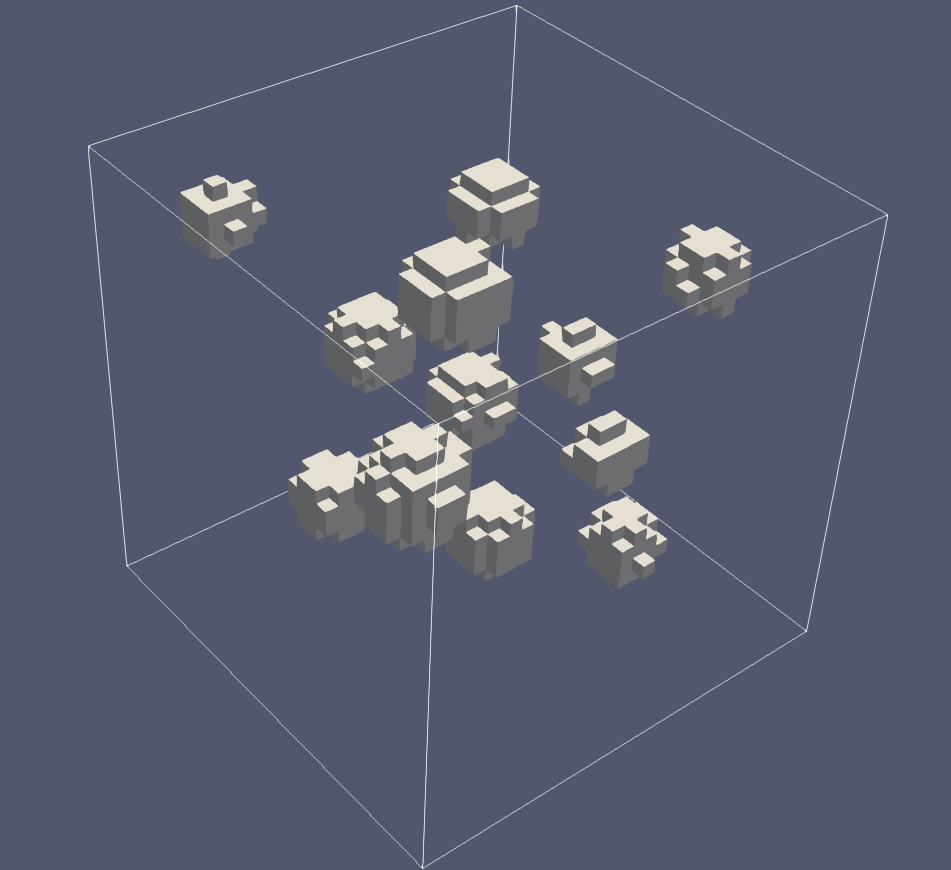
\includegraphics[width=0.72\textwidth]{../result/plots/mu.png}
\caption{Cellwise visualization of the coefficient field for $p=5$. Orange inclusions have
$\mu=10^5$ and the background has $\mu=1$. The apparent faceting comes from evaluation on the
uniform hexahedral mesh.}
\label{fig:mu}
\end{figure}

With $f=1$, the solution is positive in the interior. High-$\mu$ regions penalize gradients more
strongly, so the solution tends to become locally flatter inside them while flux continuity couples
them to the background. Algebraically, element contributions in the inclusions are scaled by
$10^p$, creating widely separated energy scales. A diagonal correction can normalize individual
rows, but it cannot fully represent the collective modes produced by separated inclusions. This is
the physical origin of the preconditioning challenge.

\newpage
\section{Robustness with respect to heterogeneity}
\begin{figure}[h]
\centering
\begin{tikzpicture}
\begin{semilogyaxis}[width=.92\textwidth,height=.53\textheight,xlabel={$p$},ylabel={CG iterations},
  xtick={1,2,3,4,5},grid=major,legend columns=3,legend style={at={(0.5,-.2)},anchor=north}]
\methodstyle{*}{nonec} table[x=p,y=none,col sep=comma]{generated/iterations_by_p.dat};\addlegendentry{none}
\methodstyle{square*}{jacobic} table[x=p,y=jacobi,col sep=comma]{generated/iterations_by_p.dat};\addlegendentry{Jacobi}
\methodstyle{triangle*}{ssorc} table[x=p,y=ssor,col sep=comma]{generated/iterations_by_p.dat};\addlegendentry{SSOR}
\methodstyle{diamond*}{iluc} table[x=p,y=ilu,col sep=comma]{generated/iterations_by_p.dat};\addlegendentry{ILU}
\methodstyle{pentagon*}{amgc} table[x=p,y=amg,col sep=comma]{generated/iterations_by_p.dat};\addlegendentry{AMG}
\end{semilogyaxis}
\end{tikzpicture}
\caption{Iteration count against contrast exponent on the finest serial mesh. Data are tabulated
in a compact derived file to keep plot filtering transparent.}
\label{fig:heterogeneity}
\end{figure}

The baseline grows from 260 iterations at $p=1$ to 16,067 at $p=5$, a factor of 61.8. Jacobi
improves the hardest case to 611 iterations, SSOR to 211, and ILU to 172, but all still degrade as
contrast rises. AMG changes only from 17 to 31 iterations, a factor of 1.82. In this operational
sense AMG is robust with respect to the tested heterogeneity, though not perfectly contrast
independent.

\newpage
\section{Spectral evidence}
\begin{figure}[h]
\centering
\begin{tikzpicture}
\begin{semilogyaxis}[width=.92\textwidth,height=.54\textheight,xlabel={$p$},ylabel={estimated condition number},
xtick={1,2,3,4,5},grid=major,legend columns=3,legend style={at={(0.5,-.2)},anchor=north}]
\methodstyle{*}{nonec} table[x=p,y=none,col sep=comma]{generated/condition_by_p.dat};\addlegendentry{none}
\methodstyle{square*}{jacobic} table[x=p,y=jacobi,col sep=comma]{generated/condition_by_p.dat};\addlegendentry{Jacobi}
\methodstyle{triangle*}{ssorc} table[x=p,y=ssor,col sep=comma]{generated/condition_by_p.dat};\addlegendentry{SSOR}
\methodstyle{diamond*}{iluc} table[x=p,y=ilu,col sep=comma]{generated/condition_by_p.dat};\addlegendentry{ILU}
\methodstyle{pentagon*}{amgc} table[x=p,y=amg,col sep=comma]{generated/condition_by_p.dat};\addlegendentry{AMG}
\end{semilogyaxis}
\end{tikzpicture}
\caption{CG/Lanczos condition estimates at $r=5$, $np=1$.}
\label{fig:condition}
\end{figure}

At $p=5$, the estimated condition numbers are $1.05\times10^7$ (none), $1.50\times10^6$
(Jacobi), $1.70\times10^5$ (SSOR), $1.13\times10^5$ (ILU), and 18.5 (AMG). The ordering mirrors
the iteration counts and supports the spectral explanation in \cref{eq:cg-bound}. AMG's estimate
stays between 2.51 and 18.5 over all five contrasts, whereas the other curves inherit a near
order-of-magnitude increase for each increment of $p$.

These are effective preconditioned condition estimates, not exact matrix condition numbers. Their
value is comparative: they show that AMG changes the spectrum qualitatively, while diagonal and
local approaches mainly reduce its scale.

\newpage
\section{Total time on the hardest serial case}
\begin{figure}[h]
\centering
\begin{tikzpicture}
\begin{axis}[ybar,width=.9\textwidth,height=.52\textheight,ymode=log,ylabel={seconds},
symbolic x coords={none,Jacobi,SSOR,ILU,AMG},xtick=data,nodes near coords,
every node near coord/.append style={font=\small,rotate=45,anchor=west},grid=major]
\addplot[fill=polimiblue!70] coordinates {(none,16.9413) (Jacobi,.361529) (SSOR,.494260) (ILU,.399305) (AMG,.262400)};
\end{axis}
\end{tikzpicture}
\caption{Preconditioner setup plus solve time for $p=5$, $r=5$, $np=1$. Logarithmic scale.}
\label{fig:serialtime}
\end{figure}

AMG is fastest overall at 0.262 s despite its nonzero setup. Relative to no preconditioner it gives
a $64.6\times$ reduction; relative to Jacobi, SSOR, and ILU it is respectively $1.38\times$,
$1.88\times$, and $1.52\times$ faster. ILU needs fewer iterations than SSOR and also finishes
sooner, while Jacobi's very cheap applications offset its much larger iteration count.

Timing very short cases is noisy, which is why the hardest case is most informative. The conclusion
is nonetheless clear at the scale of the baseline gap: iteration robustness is large enough to repay
AMG construction. For repeated solves with the same matrix, reusing the AMG hierarchy would make
its advantage stronger than the one-shot totals shown here.

\newpage
\section{Setup and solve cost decomposition}
\begin{figure}[h]
\centering
\begin{tikzpicture}
\begin{axis}[ybar stacked,width=.9\textwidth,height=.52\textheight,ylabel={seconds},ymin=0,
symbolic x coords={Jacobi,SSOR,ILU,AMG},xtick=data,legend style={at={(.5,-.18)},anchor=north,legend columns=2},grid=major]
\addplot[fill=amgc] coordinates {(Jacobi,.00228942) (SSOR,.00173475) (ILU,.0439936) (AMG,.0864544)};
\addplot[fill=nonec] coordinates {(Jacobi,.359240) (SSOR,.492525) (ILU,.355311) (AMG,.175946)};
\legend{setup,solve}
\end{axis}
\end{tikzpicture}
\caption{Cost decomposition at $p=5$, $r=5$, $np=1$.}
\label{fig:split}
\end{figure}

AMG spends 33\% of its total in setup, ILU 11\%, and Jacobi/SSOR below 1\%. AMG nevertheless has
the shortest solve phase because its 31 iterations are substantially more productive. SSOR is a
notable counterexample to ``cheap setup means cheap solve'': its relaxation setup is negligible,
but 211 communication- and ordering-sensitive iterations cost almost half a second.

The right metric depends on reuse. If $m$ right-hand sides share a matrix and the preconditioner is
reused, average cost becomes $t_{setup}/m+t_{solve}$. Conversely, if matrices change every step,
setup is paid repeatedly. The benchmark reports both components precisely so this application-level
tradeoff can be reconstructed rather than hidden in a single number.

\newpage
\section{Mesh dependence and algorithmic optimality}
\begin{figure}[h]
\centering
\begin{tikzpicture}
\begin{semilogyaxis}[width=.92\textwidth,height=.54\textheight,xlabel={global refinement $r$},ylabel={CG iterations},
xtick={3,4,5},grid=major,legend columns=3,legend style={at={(.5,-.2)},anchor=north}]
\methodstyle{*}{nonec} table[x=r,y=none,col sep=comma]{generated/iterations_by_ref.dat};\addlegendentry{none}
\methodstyle{square*}{jacobic} table[x=r,y=jacobi,col sep=comma]{generated/iterations_by_ref.dat};\addlegendentry{Jacobi}
\methodstyle{triangle*}{ssorc} table[x=r,y=ssor,col sep=comma]{generated/iterations_by_ref.dat};\addlegendentry{SSOR}
\methodstyle{diamond*}{iluc} table[x=r,y=ilu,col sep=comma]{generated/iterations_by_ref.dat};\addlegendentry{ILU}
\methodstyle{pentagon*}{amgc} table[x=r,y=amg,col sep=comma]{generated/iterations_by_ref.dat};\addlegendentry{AMG}
\end{semilogyaxis}
\end{tikzpicture}
\caption{Iteration count versus mesh refinement for $p=5$, $np=1$.}
\label{fig:optimality}
\end{figure}

From $r=3$ to 5, DoFs grow by a factor of 49.3. Iterations grow from 1,031 to 16,067 without a
preconditioner; from 296 to 611 with Jacobi; from 124 to 211 with SSOR; and from 103 to 172 with
ILU. AMG rises from an anomalous one-step coarse solve to 31 iterations, with 64 iterations at
$r=4$ and 31 at $r=5$; therefore the three-point sequence is not monotone.

Strict $h$-optimality would mean an iteration count bounded independently of refinement. The data
do not establish that asymptotic property for any method, because only three modest meshes are
tested and AMG defaults can produce coarse-grid artifacts. Still, on the two resolved meshes AMG
keeps counts in the tens while the baseline reaches thousands. We describe it as the strongest
evidence of practical mesh robustness, not as a proof of optimal complexity.

\newpage
\section{Strong scaling}
\begin{figure}[h]
\centering
\begin{tikzpicture}
\begin{axis}[width=.92\textwidth,height=.54\textheight,xlabel={MPI processes},ylabel={speedup $T(1)/T(np)$},
xtick={1,2,3,4},grid=major,legend columns=3,legend style={at={(.5,-.2)},anchor=north}]
\addplot[dashed,thick,color=black] coordinates {(1,1)(2,2)(3,3)(4,4)};\addlegendentry{ideal}
\methodstyle{*}{nonec} table[x=np,y=none,col sep=comma]{generated/speedup_by_np.dat};\addlegendentry{none}
\methodstyle{square*}{jacobic} table[x=np,y=jacobi,col sep=comma]{generated/speedup_by_np.dat};\addlegendentry{Jacobi}
\methodstyle{triangle*}{ssorc} table[x=np,y=ssor,col sep=comma]{generated/speedup_by_np.dat};\addlegendentry{SSOR}
\methodstyle{diamond*}{iluc} table[x=np,y=ilu,col sep=comma]{generated/speedup_by_np.dat};\addlegendentry{ILU}
\methodstyle{pentagon*}{amgc} table[x=np,y=amg,col sep=comma]{generated/speedup_by_np.dat};\addlegendentry{AMG}
\end{axis}
\end{tikzpicture}
\caption{Strong scaling at $p=5$, $r=5$. Values include preconditioner setup and solve.}
\label{fig:scaling}
\end{figure}

At four ranks the measured speedups are 2.45 (none), 2.06 (Jacobi), 0.72 (SSOR), 2.28 (ILU),
and 1.57 (AMG). SSOR becomes slower, consistent with relaxation dependencies and a small
per-rank workload. AMG remains the fastest absolute method at four ranks (0.168 s), narrowly ahead
of Jacobi and ILU, even though its speedup is not the best.

The $np=2$ results contain pronounced timing anomalies for several methods; $np=3$ and 4 are
often faster. This nonmonotonicity signals that single short runs do not isolate parallel performance
cleanly. Repeated trials and larger meshes are needed before drawing hardware-level conclusions.

\newpage
\section{Quantitative synthesis}
\begin{table}[h]
\centering
\caption{Hardest-case summary ($p=5$, $r=5$). Speedup compares one and four ranks.}
\small
\begin{tabular}{lrrrrr}
\toprule
Method & iter. (1 rank) & $\widehat\kappa$ & $T_1$ [s] & $T_4$ [s] & $S_4$\\
\midrule
None   & 16,067 & $1.051\times10^7$ & 16.941 & 6.922 & 2.45\\
Jacobi & 611    & $1.504\times10^6$ & 0.362  & 0.175 & 2.06\\
SSOR   & 211    & $1.701\times10^5$ & 0.494  & 0.683 & 0.72\\
ILU    & 172    & $1.133\times10^5$ & 0.399  & 0.175 & 2.28\\
AMG    & 31     & $1.847\times10^1$ & 0.262  & 0.168 & 1.57\\
\bottomrule
\end{tabular}
\label{tab:synthesis}
\end{table}

\begin{table}[h]
\centering
\caption{Decision-oriented comparison supported by the measured regime.}
\begin{tabularx}{\textwidth}{lXXX}
\toprule
Method & Principal strength & Principal weakness & Appropriate use\\
\midrule
None & zero overhead & catastrophic contrast sensitivity & baseline only\\
Jacobi & simple and parallel & weak spectral correction & cheap moderate cases\\
SSOR & fewer serial iterations & poor observed scaling & small serial/subdomain use\\
ILU & strong local correction & triangular dependencies & moderate rank count\\
AMG & best spectral robustness & hierarchy/coarse overhead & difficult elliptic systems\\
\bottomrule
\end{tabularx}
\end{table}

No single column should be read in isolation. The unpreconditioned solve has better four-rank
speedup than AMG but remains 41 times slower there. SSOR has fewer iterations than Jacobi but a
longer serial runtime and negative scaling. AMG wins the primary objective because it combines the
lowest hard-case time with by far the smallest condition estimate and mild contrast sensitivity.

\newpage
\section{Discussion}
Three mechanisms explain the main results. First, high contrast creates modes whose energy is
localized around inclusion interfaces. Jacobi sees only nodal scale, so it cannot eliminate their
collective coupling. Second, SSOR and ILU capture richer local structure, explaining their substantial
serial improvement, but distributed subdomains interrupt what would otherwise be global sweeps or
factors. Third, AMG explicitly transfers smooth error to coarse spaces, which attacks the global
component that local methods leave behind.

The results also distinguish four meanings of ``best'':
\begin{itemize}
 \item \emph{effectiveness}: iteration and condition-number reduction;
 \item \emph{efficiency}: setup plus solve wall time;
 \item \emph{optimality}: bounded work growth under mesh refinement;
 \item \emph{scalability}: reduced time as ranks are added to a fixed problem.
\end{itemize}
AMG leads the first two and provides the best practical evidence for the third, while its measured
strong scaling is only moderate. Jacobi and the baseline expose more parallel work per solve and can
therefore show respectable speedup, but speed up a much worse algorithm. The appropriate comparison
is absolute time at a specified accuracy, with speedup as a secondary diagnostic.

An initially surprising feature is that AMG takes one iteration for all $p$ on the coarsest mesh.
This likely means the automatically built hierarchy or coarse solve nearly reproduces the tiny
system; the missing condition estimate is consistent with an insufficient Lanczos history. Those
points should not be interpreted as general one-iteration convergence. The finer meshes provide the
credible robustness evidence.

\newpage
\section{Limitations and recommended extensions}
The study is complete for the specified parameter grid, but its scope imposes limitations.
\begin{enumerate}
 \item Each timing appears to be a single observation. Repeating cases, reporting medians and
 dispersion, pinning processes, and recording hardware would make performance claims stronger.
 \item The largest system has only 35,937 DoFs. Strong-scaling saturation therefore arrives early;
 million-DoF meshes would better expose parallel asymptotics.
 \item Only default preconditioner settings are used. AMG smoothers, aggregation thresholds,
 coarse solvers, ILU fill, overlap, and relaxation parameters deserve controlled tuning.
 \item The spheres are unfitted. A mesh-aligned or adaptively refined interface study would separate
 geometry error from algebraic difficulty.
 \item Estimated condition numbers come from CG and are unavailable for one-step cases. A small
 eigenvalue study on representative systems would provide independent spectral validation.
\end{enumerate}

Reproducibility also benefits from preserving the raw CSV, exact source revision, deal.II/Trilinos
versions, compiler flags, MPI implementation, node topology, and launch command. The repository
already includes the executable modes and automation needed to regenerate the principal outputs.
The most valuable next experiment is a repeated strong- and weak-scaling campaign on larger grids,
followed by AMG parameter sensitivity at $p=5$. This would test whether the current qualitative
ranking persists when communication is amortized by substantial local work.

\newpage
\section{Conclusions}
The finite-element implementation is verified: the manufactured solution achieves the theoretical
$Q_1$ rates of two in $L^2$ and one in $H^1$. The production sweep then demonstrates that
coefficient heterogeneity, not merely mesh size, is the decisive algebraic challenge. Without
preconditioning, the hardest system requires 16,067 CG iterations and has an estimated condition
number above $10^7$.

All four preconditioners help, but their quality differs. Jacobi is inexpensive and parallel but not
contrast robust. SSOR and ILU make stronger local corrections; ILU is generally the more attractive
of these two in total time, while SSOR scales poorly in the tested distributed setting. AMG changes
the outcome qualitatively: 31 iterations, an estimated condition number of 18.5, and the smallest
serial and four-rank total times for the hardest case.

Accordingly, \textbf{AMG is the recommended default for this heterogeneous elliptic problem}.
That conclusion is based on absolute efficiency and spectral robustness, not on speedup alone.
For very small or mildly heterogeneous systems, Jacobi can remain reasonable because setup is
negligible. ILU is a competitive intermediate choice when a multigrid hierarchy is undesirable.

The broader lesson is methodological. Solver assessment must keep discretization verification,
iteration robustness, setup/solve decomposition, mesh dependence, and parallel scaling distinct.
The 300-case dataset supports all five views and prevents a superficially good metric from hiding a
poor end-to-end method.

\newpage
\section{Bibliography}
\begin{thebibliography}{9}
\bibitem{quarteroni2017}
A. Quarteroni,
\emph{Numerical Models for Differential Problems}, 3rd ed.
Springer, 2017.

\bibitem{saad2003}
Y. Saad,
\emph{Iterative Methods for Sparse Linear Systems}, 2nd ed.
SIAM, 2003.

\bibitem{trottenberg2001}
U. Trottenberg, C. W. Oosterlee, and A. Sch\"uller,
\emph{Multigrid}. Academic Press, 2001.

\bibitem{smith1996}
B. F. Smith, P. E. Bj\o rstad, and W. D. Gropp,
\emph{Domain Decomposition: Parallel Multilevel Methods for Elliptic PDEs}.
Cambridge University Press, 1996.

\bibitem{dealii2020}
D. Arndt et al., ``The deal.II Library, Version 9.2,''
\emph{Journal of Numerical Mathematics}, 28(3), pp. 131--146, 2020.

\bibitem{trilinos2005}
M. A. Heroux et al., ``An overview of the Trilinos project,''
\emph{ACM Transactions on Mathematical Software}, 31(3), pp. 397--423, 2005.

\bibitem{projectbrief}
NMPDE teaching staff, ``Project 1: Preconditioning heterogeneous diffusion problems,''
Numerical Methods for Partial Differential Equations, A.Y. 2025/2026.

\bibitem{repository}
Project source repository, \url{https://github.com/DOCCA0/nmpde-projects}, accessed 2026.
\end{thebibliography}

\vfill
\small
\textbf{Data availability.} The complete 300-row dataset is stored in
\texttt{result/benchmark\_results.csv}. The implementation and benchmark driver are included in
the repository. This report was typeset directly with LaTeX; run \texttt{latexmk -pdf report.tex}
to regenerate it.

\end{document}
